% Copyright 2026 Fausto Spoto
%
% Licensed under the Apache License, Version 2.0 (the "License");
% you may not use this file except in compliance with the License.
% You may obtain a copy of the License at
%
%    http://www.apache.org/licenses/LICENSE-2.0
%
% Unless required by applicable law or agreed to in writing, software
% distributed under the License is distributed on an "AS IS" BASIS,
% WITHOUT WARRANTIES OR CONDITIONS OF ANY KIND, either express or implied.
% See the License for the specific language governing permissions and
% limitations under the License.

\documentclass[11pt]{beamer}  %% versione proiettore
%%\documentclass[11pt,handout]{beamer} %% versione stampa
\usepackage{lucidiJb-2ed}

\usepackage{mathtools}
\usepackage{relsize}
\usepackage[normalem]{ulem}
\usepackage[dvipsnames]{xcolor}
\usepackage{amsmath}
\usepackage{amssymb}
\usepackage{tikz}
\usetikzlibrary{decorations.pathreplacing}

\mode<article>
{
  \usepackage{fullpage}
  \usepackage{hyperref}
}

\mode<presentation>
{
  \setbeamertemplate{background canvas}[vertical shading][bottom=red!10,top=blue!10]
  \usetheme{Course}
  \usefonttheme[onlysmall]{structurebold}
}

\newcommand{\wrt}{\textit{wrt.\ }}
\newcommand{\ie}{, \textit{ie.}, }
\newcommand{\iestart}{\textit{ie.}, }

\newcommand{\numberofscoops}{{\#\mathit{scoops}}}
\newcommand{\noncesize}{{\mathit{nonce}_{\mathit{size}}}}
\newcommand{\byte}{{\mathit{byte}}}
\newcommand{\nonce}{{\mathit{nonce}}}
\newcommand{\nonces}{{\mathit{nonces}}}
\newcommand{\scoops}{{\mathit{scoops}}}
\newcommand{\plot}{{\mathit{plot}}}
\newcommand{\scoop}{{\mathit{scoop}}}
\newcommand{\seed}{{\mathit{seed}}}
\newcommand{\previous}{{\mathit{previous}}}
\newcommand{\deadline}{{\mathit{deadline}}}
\newcommand{\public}{{\mathit{public}}}
\newcommand{\chainid}{{\mathit{chainId}}}
\newcommand{\generation}{{\mathit{generation}}}
\newcommand{\size}{{\mathit{size}}}
\newcommand{\scoopnumber}{{\mathit{scoopNumber}}}
\newcommand{\data}{{\mathit{data}}}
\newcommand{\challenge}{{\mathit{challenge}}}
\newcommand{\delay}{{\mathit{delay}}}
\newcommand{\mynext}{{\mathit{next}}}
\newcommand{\nextchallenge}{\challenge_\mynext}
\newcommand{\initialchallenge}{{\mathit{initialChallenge}}}
\newcommand{\height}{{\mathit{height}}}
\newcommand{\trunk}{{\mathit{trunk}}}
\renewcommand{\block}{{\mathit{block}}}
\newcommand{\oblivion}{{\mathit{oblivion}}}
\newcommand{\now}{{\mathit{now}}}
\newcommand{\beat}{{\mathit{beat}}}
\newcommand{\weightedbeat}{\mathit{weightedBeat}}
\newcommand{\nextweightedbeat}{\weightedbeat_\mynext}
\newcommand{\power}{{\mathit{power}}}
\newcommand{\hash}{{\mathit{hash}}}
\newcommand{\difficulty}{{\mathit{difficulty}}}
\newcommand{\hashfirstk}{{\mathit{hash\ of\ first\ \kappa\ bytes\ of}}}
\newcommand{\previousblockhash}{{\mathit{previousBlockHash}}}
\newcommand{\waitingtime}{{\mathit{waitingTime}}}
\newcommand{\nextwaitingtime}{\tau_\mynext}
\newcommand{\nextpower}{\power_\mynext}
\newcommand{\nextacceleration}{\alpha_\mynext}
\newcommand{\nextblock}{\block_\mynext}
\newcommand{\genesis}{{\mathit{genesis}}}
\newcommand{\consensus}{{\mathit{consensus}}}
\newcommand{\nattobe}{{\mathit{nat2be}}}
\newcommand{\betonat}{{\mathit{be2nat}}}
\newcommand{\finalhash}{{h_{\mathit{final}}}}
\newcommand{\chainidentifier}{{\mathit{chainIdentifier}}}
\newcommand{\publickeyofpeer}{{\mathit{publicKeyOfPeer}}}
\newcommand{\publickeyofminer}{{\mathit{publicKeyOfMiner}}}

\newcommand{\Prologs}{{\mathsf{Prologs}}}
\newcommand{\Plots}{{\mathsf{Plots}}}
\newcommand{\Challenges}{{\mathsf{Challenges}}}
\newcommand{\Scoops}{{\mathsf{Scoops}}}
\newcommand{\Nonces}{{\mathsf{Nonces}}}
\newcommand{\Trunks}{{\mathsf{Trunks}}}
\newcommand{\Blocks}{{\mathsf{Blocks}}}
\newcommand{\GenesisBlocks}{{\mathsf{GenesisBlocks}}}
\newcommand{\NonGenesisBlocks}{{\mathsf{NonGenesisBlocks}}}
\newcommand{\Deadlines}{{\mathsf{Deadlines}}}
\DeclareMathOperator*{\append}{\bowtie}

\subtitle{DLT2026 – 8th Distributed Ledger Technology Workshop, Pula, Italy, June 2026}
\title{Mobile Mining\\for Proof of Space}
\institute{Universit\`a di Verona, Italy}
\date{June 2026}

\setbeamercovered{invisible}

\def\codesize{\smaller}
\def\<#1>{\codeid{#1}}
\newcommand{\codeid}[1]{\ifmmode{\mbox{\codesize\ttfamily{#1}}}\else{\codesize\ttfamily #1}\fi}

\AtBeginSection[]{
  \begin{frame}
  \vfill
  \centering
  \begin{beamercolorbox}[sep=8pt,center,shadow=true,rounded=true]{title}
    \usebeamerfont{title}\insertsectionhead\par%
  \end{beamercolorbox}
  \vfill
  \end{frame}
}

\colorlet{lightred}{red!50!white}
\colorlet{verylightred}{red!20!white}
\colorlet{verylightyellow}{yellow!20!white}
\colorlet{verylightviolet}{violet!20!white}
\colorlet{verylightgreen}{green!20!white}
\colorlet{verylightgray}{gray!20!white}

\newcommand{\db}{
\includegraphics[width=1.3cm]{pictures/db}}
\newcommand{\computer}{
\includegraphics[width=1.3cm]{pictures/computer}}
\newcommand{\phone}{
\includegraphics[width=1.3cm]{pictures/phone}}

\begin{document}

\begin{frame}
  \titlepage
\end{frame}

\begin{frame}
  \frametitle{Wo decides the next block?}

  \begin{greenbox}{Many alternatives}
    \begin{itemize}
    \item Proof of Work [PoW] (who commits more work)
    \item Proof of Stake [PoS] (who commits more money)
    \item Proof of Authority [PoA] (who has more authority)
    \item Proof of Space [PoSp] (who commits more disk space)
    \item \ldots
    \end{itemize}
  \end{greenbox}

  \bigskip
  
  \begin{greenbox}{Proof of Space is an interesting, niche technology}
  \begin{itemize}
  \item fully decentralized
  \item no CPU cost
  \item no \emph{special} nodes (no validators)
  \item miners join and leave anonymously
  \end{itemize}
  \end{greenbox}

\end{frame}

\begin{frame}{Blockchain mining as a competitive puzzle}

  \visible<1->{Bitcoin's Proof of Work:}
  \begin{description}
  \item<2->[{\color{red}challenge:}] find a \textbf{next} such that $\hash(\mathbf{next})>\difficulty$
  \item<3->[{\color{red}answer:}] reply with a \textbf{next} obtained
    by rotating all possible values of an unused field \emph{nonce}, until $\hash(\mathbf{next})>\difficulty$
  \item<4->[{\color{red}competition:}] in case of more \textbf{next}, select the one with the largest hash
  \end{description}

\end{frame}

\begin{frame}\frametitle{A Bitcoin (or old Ethereum) node and its miner(s)}

  \begin{center}
    \begin{tikzpicture}[scale=1]
      \draw [fill=verylightviolet,thick] (-0.5,-1.5) rectangle +(4,3);
      \draw (1.5,0.8) node {blockchain peer};
      \draw (1.5,0.4) node {{\small (networking \& consensus)}};
      \draw[-, thick] (1.5,-1.5) -- (1.5,-2.7);
      \draw (1.5,-2.7) node[scale=0.7] {\db};
      \draw (3.7,-2.7) node {database of blocks};
      \draw[<->, thick] (3.5,-1) -- (5.5,-1);
      \draw (6.6,-1) node {other peers};
      \draw (4.5,-1.2) node {{\scriptsize gossiping}};

      \draw [fill=verylightyellow,thick] (0.5,-0.7) rectangle +(2,0.5);
      \draw (1.5,-0.45) node {mempool};
      \draw[->, thick] (-1.5,-0.45) -- (0.5,-0.45);
      \draw (-2.3,-0.45) node {requests};

      \draw [fill=verylightred,thick] (7,0.35) rectangle +(2,0.8);
      \draw (8.0,0.75) node {miner(s)};

      \draw [fill=verylightgreen,thick] (0.5,3) rectangle +(2,0.8);
      \draw (1.5,3.4) node {application};
      \draw[-, thick] (0.5,3.4) -- (-1,3.4);
      \draw (-1,3.4) node[scale=0.7] {\db};
      \draw (-1,2.5) node {database of states};

      \draw[->, thick] (3.5,1.0) -- (7,1.0);
      \draw (5.25,1.2) node {{\small challenges (blocks)}};

      \draw[<-, thick] (3.5,0.5) -- (7,0.5);
      \draw (5.25,0.25) node {{\small answers (nonces)}};
      %\draw (5.25,0) node {{\scriptsize (in this paper, nonces or deadlines)}};

      \draw[->, thick] (1.2,1.5) -- (1.2,3);
      \draw[->, thick] (1.8,3) -- (1.8,1.5);
      \draw (1.5,2.25) node {{\small API}};
    \end{tikzpicture}
  \end{center}

\end{frame}

\begin{frame}\frametitle{Miners as mobile applications}

  \begin{center}
    \begin{tikzpicture}[scale=1]
      \draw [fill=verylightviolet,thick] (-0.5,0) rectangle +(4,1.5);
      \draw (1.5,0.8) node {blockchain peer};
      \draw (1.5,2.2) node[scale=0.7] {\computer};
      \draw (-1.5,0.8) node[scale=0.7] {\db};

      \draw [fill=verylightred,thick] (7,0.35) rectangle +(2,0.8);
      \draw (8.0,0.75) node {miner(s)};
      \draw (8.0,2) node[scale=0.7] {\phone};

      \draw[->, thick] (3.5,1.0) -- (7,1.0);
      \draw (5.25,1.2) node {{\small challenges (blocks)}};

      \draw[<-, thick] (3.5,0.5) -- (7,0.5);
      \draw (5.25,0.25) node {{\small answers (nonces)}};

    \end{tikzpicture}
  \end{center}

  \smallskip

  \begin{center}
    \alert{Why a mobile application?}
  \end{center}

  \pause

  \begin{itemize}
  \item mobile devices are a huge already existing hardware base
  \item a mobile application could introduce mining to a large portion of humanity, who owns a
    phone but not a powerful connected computer
  \item it can be easily and automatically  updated
  \item it simplifies the start-up of new blockchains
  \item it has educational and marketing relevance
  \end{itemize}

\end{frame}

\begin{frame}\frametitle{Miners as mobile applications}

  \begin{center}
    \begin{tikzpicture}[scale=1]
      \draw [fill=verylightviolet,thick] (-0.5,0) rectangle +(4,1.5);
      \draw (1.5,0.8) node {blockchain peer};
      \draw (1.5,2.2) node[scale=0.7] {\computer};
      \draw (-1.5,0.8) node[scale=0.7] {\db};

      \draw [fill=verylightred,thick] (7,0.35) rectangle +(2,0.8);
      \draw (8.0,0.75) node {miner(s)};
      \draw (8.0,2) node[scale=0.7] {\phone};

      \draw[->, thick] (3.5,1.0) -- (7,1.0);
      \draw (5.25,1.2) node {{\small challenges (blocks)}};

      \draw[<-, thick] (3.5,0.5) -- (7,0.5);
      \draw (5.25,0.25) node {{\small answers (nonces)}};

    \end{tikzpicture}
  \end{center}

  \medskip

  \begin{center}
    \alert{Can we do it for PoW (Bitcoin or old Ethereum) ?}
  \end{center}

  \pause

  \begin{itemize}
  \item no, since PoW is a CPU intensive computation
    \begin{itemize}
    \item mobile devices are not competitive for that
    \item their battery would immediately die
    \end{itemize}
  \item no, since blocks are too large for being streamed to a mobile
    \begin{itemize}
    \item mobile networks are relatively slow
    \item data packages are still very limited for that
    \end{itemize}
  \end{itemize}

\end{frame}

\begin{frame}\frametitle{Enter Proof of Space}

  \begin{greenbox}{}
    \begin{itemize}
    \item Ateniese, Bonacina, Faonio, Galesi: \emph{Proofs of Space: When Space Is of the Essence}, 2014 (DAG pebbling)
    \item Dziembowski, Faust, Kolmogorov, Pietrzak: \emph{Proofs of Space}, 2015 (DAG pebbling) $\Rightarrow$
      {\color{red}SpaceMint}: \url{https://github.com/kwonalbert/spacemint}
    \item Abusalah, Alwen, Cohen, Khilko, Pietrzak, Reyzin: \emph{Beyond Hellman's Time-Memory Trade-Offs with Applications to Proofs of Space}, 2017 (proof of sequential work + proof of space) $\Rightarrow$ {\color{red}Chia}: \url{https://www.chia.net/wp-content/uploads/2022/07/ChiaGreenPaper.pdf}
    \item \emph{Signum Community Website and Documentation Project} (plot files) $\Rightarrow$ {\color{red}Signum}: \url{https://wiki.signum.network}
    \end{itemize}

  \begin{center}
    {\small\begin{tabular}{c|c|c|c|c|c}
      tool & consensus & network & formalized & since & status \\\hline\hline
      SpaceMint & no & no & yes & 2015 & discontinued\\\hline
      Chia & yes & yes & yes & 2017 & active\\\hline
      Signum & yes & yes & \alert{no} & 2014 & active\\\hline
    \end{tabular}}
  \end{center}
  \end{greenbox}
  
\end{frame}

\begin{frame}{From Signum to Mokamint}

  \begin{itemize}
  \item possibly the first ever smart contracts (before Ethereum!)
  \item commercial web page: \url{https://signum.network/}
  \item very informal documentation: \url{https://wiki.signum.network}
  \item chaotic, uncommented, monolithic code:
    \url{https://github.com/signum-network/signum-node}
  \end{itemize}

  \bigskip

  \begin{greenbox}{}
    Fausto Spoto: \emph{A Formalization of Signum's Consensus},
    9th Workshop on Trusted Smart Contracts, Miyakojima, Japan, April 2025, LNCS 15753

    \medskip

    Fausto Spoto: \emph{\alert{Mokamint}: Generic Energy-Efficient Consensus without Validators},
    submitted for publication, 2026
  \end{greenbox}

\end{frame}

\begin{frame}\frametitle{Mokamint's plotting phase}
  \begin{center}
    It builds a plot $\nonce_0,\ldots,\nonce_{n-1}$
    for a peer, a miner and a chain\\
    \alert{it must be slow and expensive}
  \end{center}

  \[\begin{array}{l}
  \pause
  \seed=\mathit{key}^{\mathit{peer}}_\public\append\mathit{key}^{\mathit{miner}}_\public\append\chainid\bowtie p\quad\text{($\bowtie$ is byte array concatenation)}\\
  \pause
  {\color{blue} h_0}=\hash(\seed)\\
  \pause
  {\color{blue} h_1}=\hash({\color{blue} h_0}\bowtie\seed)\\
  \pause
  {\color{blue} h_2}=\hash({\color{blue} h_1}\bowtie{\color{blue}  h_0}\bowtie \seed)\\
  \pause
  \vdots\\
  {\color{blue} h_{8191}}=\hash({\color{blue} h_{8190}}\bowtie{\color{blue} h_{8189}}\bowtie\cdots\bowtie{\color{blue} h_1}\bowtie{\color{blue} h_0}\bowtie \seed)\\
  \pause
  {\color{red}\finalhash}=\hash({\color{blue} h_{8191}}\bowtie{\color{blue} h_{8190}}\bowtie\cdots\bowtie{\color{blue} h_1}\bowtie{\color{blue} h_0}\bowtie \seed)\\
  \pause
  \text{reassign }{\color{blue} h_i}={\color{blue} h_i}\oplus{\color{red}\finalhash}\text{ for every }0\le i<8192\quad\text{($\oplus$ is byte array xor)}\\
  \end{array}\]

  \pause

  \[
  \nonce_p=\underbrace{{\color{blue}h_0},{\color{blue}h_{8191}}}_{\scoop_0},\underbrace{{\color{blue}h_2},{\color{blue}h_{8189}}}_{\scoop_1},\ldots,\underbrace{{\color{blue}h_{8188}},{\color{blue}h_3}}_{\scoop_{n-2}},\underbrace{{\color{blue}h_{8190}},{\color{blue}h_1}}_{\scoop_{n-1}}
  \]

  \pause
  \begin{center}
    $\hash$ must be expensive (for instance: shabal256)
  \end{center}

\end{frame}

\begin{frame}\frametitle{Mokamint's mining phase}

  \begin{center}
    It answers a challenge $\langle i,\gamma\rangle$ derived from the topmost block of the chain\\
    \alert{it must be cheap and quick}
  \end{center}

  \smallskip

  \begin{center}
    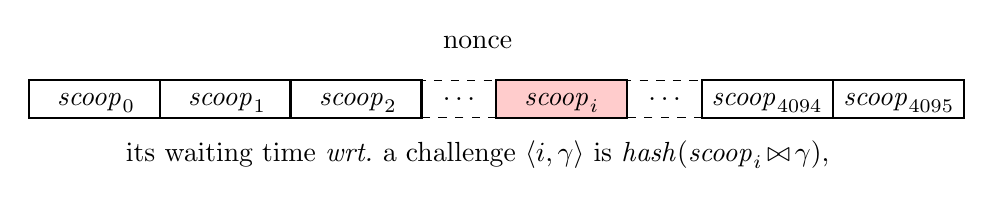
\begin{tikzpicture}[scale=0.95]

      \draw (-5.5,1) node {nonce};
      %\draw (-11.8,0.25) node {$\langle p,$};
      \draw [thick] (-11.5,0) rectangle +(1.75,0.5);
      \draw (-10.6,0.2) node {$\scoop_0$};
      \draw [thick] (-9.75,0) rectangle +(1.75,0.5);
      \draw (-8.85,0.2) node {$\scoop_1$};
      \draw [thick] (-8,0) rectangle +(1.75,0.5);
      \draw (-7.1,0.2) node {$\scoop_2$};
      \draw [dashed] (-6.25,0) rectangle +(1,0.5);
      \draw (-5.75,0.25) node {$\ldots$};
      \draw [thick,fill=verylightred] (-5.25,0) rectangle +(1.75,0.5);
      \draw (-4.375,0.2) node {$\scoop_i$};
      \draw [dashed] (-3.5,0) rectangle +(1,0.5);
      \draw (-3,0.25) node {$\ldots$};
      \draw [thick] (-2.5,0) rectangle +(1.75,0.5);
      \draw (-1.63,0.2) node {$\scoop_{4094}$};
      \draw [thick] (-0.75,0) rectangle +(1.75,0.5);
      \draw (0.13,0.2) node {$\scoop_{4095}$};
      %\draw (1.2,0.25) node {$\rangle$};

      \draw (-5.5,-0.5) node {its waiting time \wrt{}a challenge $\langle i,\gamma\rangle$ is $\hash(\scoop_i\append\gamma)$,};

    \end{tikzpicture}
  \end{center}

  \smallskip

  \begin{center}
    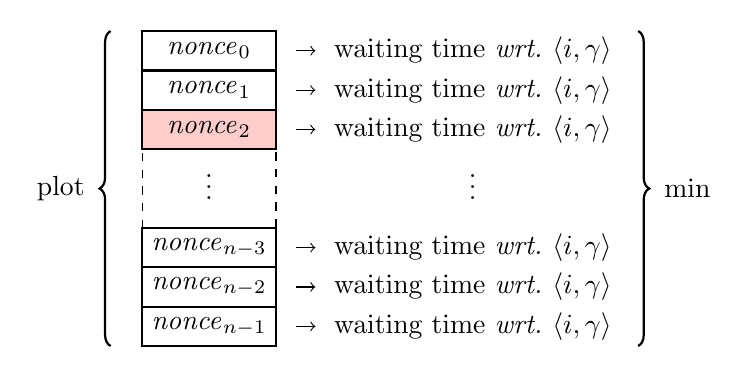
\begin{tikzpicture}[scale=1]

      \draw [decorate,decoration={brace,amplitude=4pt},thick,xshift=-0.1cm,yshift=0pt]
      (-0.5,1) -- (-0.5,5) node [midway,left,xshift=-.2cm] {plot};

      \draw [thick] (-0.2,4.5) rectangle +(1.7,0.5);
      \draw (0.65,4.75) node {$\nonce_0$};
      \draw[->] (1.75,4.75) -- +(0.25,0);
      \draw (4,4.75) node {waiting time \wrt{}$\langle i,\gamma\rangle$};

      \draw [thick] (-0.2,4) rectangle +(1.7,0.5);
      \draw (0.65,4.25) node {$\nonce_1$};
      \draw[->] (1.75,4.25) -- +(0.25,0);
      \draw (4,4.25) node {waiting time \wrt{}$\langle i,\gamma\rangle$};

      \draw [thick,fill=verylightred] (-0.2,3.5) rectangle +(1.7,0.5);
      \draw (0.65,3.75) node {$\nonce_2$};
      \draw[->] (1.75,3.75) -- +(0.25,0);
      \draw (4,3.75) node {waiting time \wrt{}$\langle i,\gamma\rangle$};

      \draw (0.65,3.125) node {$\vdots$};
      \draw [dashed] (-0.2,2.5) rectangle +(1.7,1);
      \draw (4,3.125) node {$\vdots$};

      \draw [thick] (-0.2,2) rectangle +(1.7,0.5);
      \draw (0.65,2.25) node {$\nonce_{n-3}$};
      \draw[->] (1.75,2.25) -- +(0.25,0);
      \draw (4,2.25) node {waiting time \wrt{}$\langle i,\gamma\rangle$};

      \draw [thick] (-0.2,1.5) rectangle +(1.7,0.5);
      \draw (0.65,1.75) node {$\nonce_{n-2}$};
      \draw[->] (1.75,1.75) -- +(0.25,0);
      \draw (4,1.75) node {waiting time \wrt{}$\langle i,\gamma\rangle$};

      \draw [thick] (-0.2,1) rectangle +(1.7,0.5);
      \draw (0.65,1.25) node {$\nonce_{n-1}$};
      \draw[->] (1.75,1.25) -- +(0.25,0);
      \draw (4,1.25) node {waiting time \wrt{}$\langle i,\gamma\rangle$};

      \draw [decorate,decoration={brace,amplitude=4pt},thick,xshift=0.1cm,yshift=0pt]
      (6,5) -- (6,1) node [midway,right,xshift=.2cm] {$\min$};

    \end{tikzpicture}
  \end{center}

\end{frame}

\begin{frame}\frametitle{Mokamint's Proof of Space}

  \visible<1->{A large plot file is preallocated on disk (only once!)}
  \smallskip

  \visible<2->{Blocks are enriched with a $\nonce$}
  \medskip

  \begin{description}
  \item<3->[{\color{red}challenge:}] given a $\challenge=\langle i,\gamma\rangle$
    derived from \textbf{block} find a block \textbf{next}
    with a $\nonce$ whose waiting time \wrt{}$\challenge$ is as small as possible
  \item<4->[{\color{red}answer:}] reply with a \textbf{next}
    that contains the $\nonce$ from the plot file that
    minimizes its waiting time \wrt{}$\challenge$
  \item<5->[{\color{red}competition:}] in case of more \textbf{next}, select the one whose
    nonce has the smallest waiting time \wrt{}$\challenge$
  \end{description}

\end{frame}

\begin{frame}\frametitle{Miners as mobile applications, again}

  \begin{center}
    \begin{tikzpicture}[scale=1]
      \draw [fill=verylightviolet,thick] (-0.5,0) rectangle +(4,1.5);
      \draw (1.5,1.1) node {blockchain peer};
      \draw (1.5,0.5) node {\textbf{Mokamint}};
      \draw (1.5,2.2) node[scale=0.7] {\computer};
      \draw (-1.5,0.8) node[scale=0.7] {\db};

      \draw [fill=verylightred,thick] (7,0.15) rectangle +(3,1.2);
      \draw (8.5,1) node {miner(s)};
      \draw (8.5,0.5) node {\textbf{Mokaminter}};
      \draw (8.5,2.1) node[scale=0.7] {\phone};

      \draw[->, thick] (3.5,1.0) -- (7,1.0);
      \draw (5.25,1.25) node {{\small challenges ($\langle i,\gamma\rangle$)}};

      \draw[<-, thick] (3.5,0.5) -- (7,0.5);
      \draw (5.25,0.25) node {{\small answers (nonces)}};

    \end{tikzpicture}
  \end{center}

  \begin{center}
    \alert{Can we do it for PoSp (Mokamint, at least) ?}
  \end{center}

  \pause

  \begin{itemize}
  \item yes, since PoSp uses almost no CPU during the mining phase
    \begin{itemize}
    \item this preserves the battery of the device
    \end{itemize}
  \item yes, since challenges are a around $64$ bytes long and nonces can be compacted into
    \emph{deadlines} of around $200$ bytes
    \begin{itemize}
    \item this limits data throughput during mining
    \end{itemize}
  \item yes, average mobile devices have around $256~GB$ of SSD, compared to
    an average of $1000~GB$ of SSD of desktop computers
    \begin{itemize}
    \item mining can be competitive on a mobile device
    \end{itemize}
  \end{itemize}
  
\end{frame}

\begin{frame}\frametitle{Experiments: plotting phase}

  \begin{center}
    \alert{it must be slow and expensive}
  \end{center}

  \medskip

  \begin{center}
    \begin{tabular}{|c|c||c|c|c|}
      \hline
      \textbf{device} & \textbf{type} & \textbf{nonces} & \textbf{size} & \textbf{time} \\\hline\hline
      Xiaomi 11 Lite 5G NE & phone & 1000 & 0.26~GB & 1m13s \\\hline
      Xiaomi 11 Lite 5G NE & phone & 5000 & 1.28~GB & 6m03s \\\hline
      Xiaomi 11 Lite 5G NE & phone & 10000 & 2.56~GB & 12m05s \\\hline\hline
      Samsung Galaxy Tab S6 Lite & tablet & 1000 & 0.26~GB & 2m15s \\\hline
      Samsung Galaxy Tab S6 Lite & tablet & 5000 & 1.28~GB & 11m12s \\\hline
      Samsung Galaxy Tab S6 Lite & tablet & 10000 & 2.56~GB & 22m21s \\\hline\hline
      Intel NUC8i5BEH & desktop & 1000 & 0.26~GB & 20s \\\hline
      Intel NUC8i5BEH & desktop & 5000 & 1.28~GB & 1m40s \\\hline
      Intel NUC8i5BEH & desktop & 10000 & 2.56~GB & 3m24s \\\hline
    \end{tabular}
    \vspace*{1ex}\\
    (today, the average plot size in the Hotmoka mainnet is $2257675$ nonces)
  \end{center}

\end{frame}

\begin{frame}\frametitle{Experiments: mining phase}

  \begin{center}
    \alert{it must be cheap and quick}
  \end{center}

  \medskip

  \begin{center}
    \hspace*{-1ex}\begin{tabular}{|c||c|c|c|c|c|}
      \hline
      \textbf{type} & \textbf{CPU} & \textbf{RAM} & \textbf{network} & \textbf{answer} & \textbf{earned crypto} \\\hline\hline
      phone & 0.56\% & 2.4\% (192~MB) & 3.36~MB & 0.207s & 373.30 mokas \\\hline
      tablet & 0.23\% & 3.5\% (140~MB) & 3.38~MB & 0.225s & 266.63 mokas \\\hline
      desktop & 0.09\% & 1.4\% (224~MB) & 3.39~MB & 0.019s & 319.95 mokas \\\hline
    \end{tabular}
    \vspace*{1ex}\\
    (one day of mining with a plot of $10000$ nonces)
  \end{center}

  \bigskip

  In the remaining $(\mathit{blockrate}-\mathbf{answer})$ seconds the miner does \alert{nothing}:
  \begin{itemize}
  \item no CPU activity
  \item no disk activity
  \end{itemize}

\end{frame}

\begin{frame}\frametitle{Conclusion}

  \begin{center}
    
\includegraphics[width=4.5cm]{pictures/mokaminter_logo}
  \end{center}

  \medskip
  Mokaminter is the only existing miner \emph{in} a mobile device

  \smallskip

  \begin{itemize}
  \item it works for any blockchain built over the Mokamint generic consensus engine
    based on PoSp, such as Hotmoka
  \item experiments with UFMA students in Brazil show that it increases
    the battery usage of just $0.27\%$ on average
  \item it works even with the free on board wifi of an international flight
  \item currently only for Android
  \end{itemize}

  \smallskip

  \begin{center}
    Install Mokaminter from Google Play and start mining for Hotmoka:
    \url{https://play.google.com/store/apps/details?id=io.mokamint.android.mokaminter}
  \end{center}

\end{frame}

\addtocounter{framenumber}{-1}

\begin{frame}\frametitle{5G coverage in Brazil}
  \begin{center}
    
\includegraphics[width=5.6cm]{pictures/5g}
  \end{center}
\end{frame}

\addtocounter{framenumber}{-1}

\begin{frame}\frametitle{Can somebody impersonate another miner?}

  The plotting phase creates nonces starting from a seed:
  \[
  \seed=\mathit{key}^{\mathit{peer}}_\public\append\mathit{key}^{\mathit{miner}}_\public\append\chainid\bowtie p  
  \]
  and everybody can do that with the public key of another miner!

  \medskip
  \begin{center}
    \alert{Is this a problem?}
  \end{center}
  \medskip
  \pause
  \begin{itemize}[<+->]
  \item if the impersonator creates good nonces (\iestart{}with minimal waiting time)
    the fees go to the impersonated miner (thank you!)
  \item if the impersonator creates bad nonces (\iestart{}with large waiting time)
    the peers will just discard them
  \item if the impersonator creates syntactically invalid nonces,
    the peers will ban its IP (goodbye!)
  \end{itemize}
  \pause
  It is also possible to sign nonces with the private key of the miner
\end{frame}

\addtocounter{framenumber}{-1}

\begin{frame}\frametitle{Proof of space: The general idea}

  \begin{description}
  \item[Ideal PoSp:] the computation of the answer can only be achieved by allocating
    a big data structure on disk (Ateniese et al., Dziembowski et al., Abusalah et al.)
    \medskip
  \item[Signum's PoSp:] the computation of the answer can also be achieved without
    allocating a big data structure on disk (precomputed \emph{nonces}),
    but in that case it becomes
    computationally so expensive (to recompute the nonces on-the-fly)
    that the explorable space of nonces, before the next block is created, is very small
  \end{description}

  \bigskip
  
  \begin{redbox}{Time/memory trade-off}
    The degradation of the space of explorable nonces should be at least linear with
    the reduction of the precomputed nonces
  \end{redbox}

\end{frame}

\addtocounter{framenumber}{-1}

\begin{frame}{Time/memory trade-off}

  \begin{redbox}{Park et al.: \emph{SpaceMint: A Cryptocurrency Based on Proofs of Space}, Financial Cryptography 2018}
    \emph{In Signum, it is possible to store $\finalhash$ only, instead of the full nonce,
    and recompute the smallest scoops from $\finalhash$
    in a cheap way that requires very little memory}
  \end{redbox}

  \bigskip

  \pause
  Not anymore: $\scoop_i=h_{2i},h_{2n-2i-1}$ depends from at least a $h_j$ with $j\ge n$ hence at
  least half of the $h_j$ must be recomputed in order to recompute \emph{any} given scoop

  \bigskip
  Signum's programmers have fixed their algorithm as reaction to Park et al.'s criticism

\end{frame}

\addtocounter{framenumber}{-1}

\begin{frame}{Blocks}
  \begin{center}
    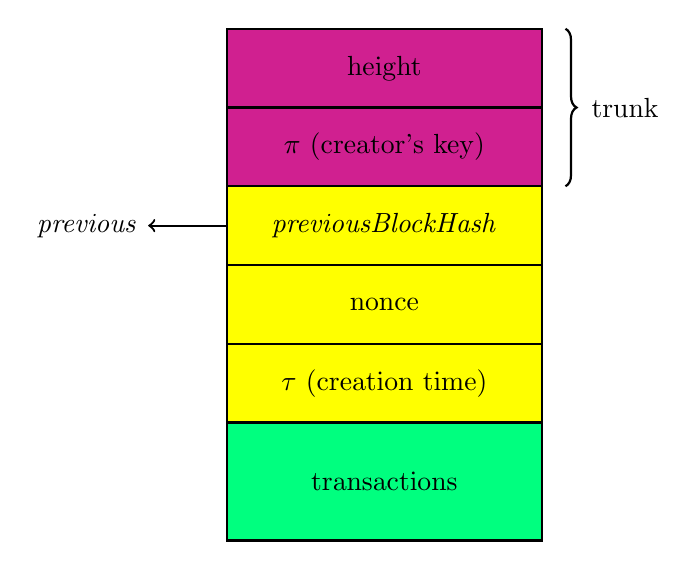
\begin{tikzpicture}
      \draw [decorate,decoration={brace,amplitude=4pt},thick,xshift=0.3cm,yshift=0pt]
      (4,6.5) -- (4,4.5) node [midway,right,xshift=.2cm] {trunk};
      \draw [fill=VioletRed, thick] (0,4.5) rectangle (4,6.5);
      \draw (2,6) node{height};
      \draw [fill=VioletRed, thick] (0,3.5) rectangle (4,5.5);
      \draw (2,5) node{$\pi$ (creator's key)};
      \draw [fill=Yellow, thick] (0,3.5) rectangle (4,4.5);
      \draw (2,4) node{$\previousblockhash$};
      \draw[->,thick] (0,4) -- (-1,4) node [midway,left,xshift=-.5cm] {$\previous$};

      \draw [fill=Yellow, thick] (0,2.5) rectangle (4,3.5);
      \draw (2,3) node{nonce};
      \draw [fill=Yellow, thick] (0,1.5) rectangle (4,2.5);
      \draw (2,2) node{$\tau$ (creation time)};

      \draw [fill=SpringGreen, thick] (0,0) rectangle (4,1.5);
      \draw (2,0.75) node{transactions};
  \end{tikzpicture}
  \end{center}
\end{frame}

\addtocounter{framenumber}{-1}

\begin{frame}[fragile]{Derivation of a challenge from a block}

  \begin{align*}
    {\color{blue}\challenge(\genesis)}&=\langle 0,\sigma_\genesis\rangle,\quad\sigma_\genesis\text{ is an arbitrary byte array}\\
    \mbox{}\\
    \visible<2->{
    {\color{blue}\challenge(\block)}&=\langle\hash(\sigma\bowtie\height)\ \mathit{mod}\ n,\sigma\rangle\\
    &\text{where $\sigma=\hash({\color{blue}\challenge(\previous)}.\sigma\bowtie\pi)$}}
  \end{align*}

  \visible<2->{
  \begin{center}
    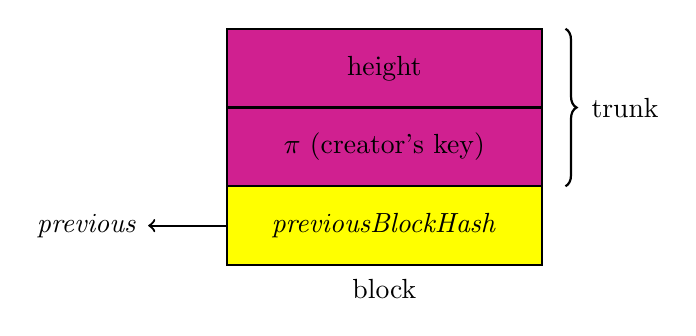
\begin{tikzpicture}
      \draw [decorate,decoration={brace,amplitude=4pt},thick,xshift=0.3cm,yshift=0pt]
      (4,7.5) -- (4,5.5) node [midway,right,xshift=.2cm] {trunk};
      \draw [fill=VioletRed, thick] (0,5.5) rectangle (4,7.5);
      \draw (2,7) node{height};
      \draw [fill=VioletRed, thick] (0,4.5) rectangle (4,6.5);
      \draw (2,6) node{$\pi$ (creator's key)};
      \draw [fill=Yellow, thick] (0,4.5) rectangle (4,5.5);
      \draw (2,5) node{$\previousblockhash$};
      \draw[->,thick] (0,5) -- (-1,5) node [midway,left,xshift=-.5cm] {$\previous$};
      \draw (2,4.2) node{block};
    \end{tikzpicture}
  \end{center}
  }

  \visible<3->{
  \begin{center}
    \textbf{Proposition.} Challenges depends on the trunks only (simple proof by induction): Signum has no block-grinding attacks
  \end{center}
  }

\end{frame}

\addtocounter{framenumber}{-1}

\begin{frame}{Miner $\pi'$ selects its best $\nonce'$ and builds a next block}

  \begin{center}
    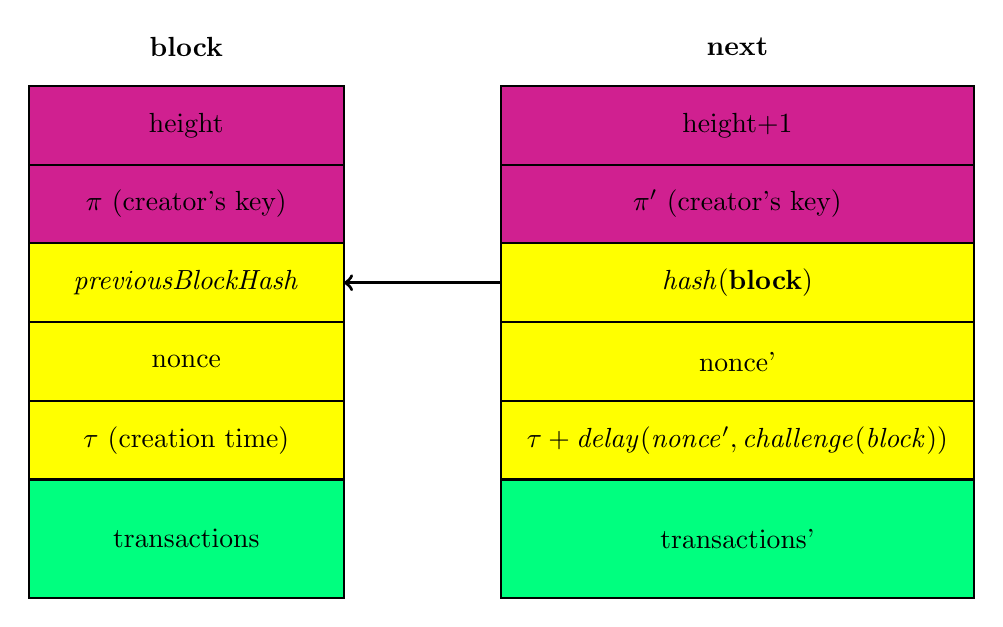
\begin{tikzpicture}
      \draw (2,7) node{\textbf{block}};
      \draw [fill=VioletRed, thick] (0,4.5) rectangle (4,6.5);
      \draw (2,6) node{height};
      \draw [fill=VioletRed, thick] (0,3.5) rectangle (4,5.5);
      \draw (2,5) node{$\pi$ (creator's key)};
      \draw [fill=Yellow, thick] (0,3.5) rectangle (4,4.5);
      \draw (2,4) node{$\previousblockhash$};

      \draw [fill=Yellow, thick] (0,2.5) rectangle (4,3.5);
      \draw (2,3) node{nonce};
      \draw [fill=Yellow, thick] (0,1.5) rectangle (4,2.5);
      \draw (2,2) node{$\tau$ (creation time)};

      \draw [fill=SpringGreen, thick] (0,0) rectangle (4,1.5);
      \draw (2,0.75) node{transactions};

      \visible<2->{
      \draw (9,7) node{\textbf{next}};
      \draw [fill=VioletRed, thick] (6,5.5) rectangle (12,6.5);
      \draw (9,6) node{height+1};
      }
      \visible<3->{
      \draw [fill=VioletRed, thick] (6,4.5) rectangle (12,5.5);
      \draw (9,5) node{$\pi'$ (creator's key)};
      }
      \visible<4->{
      \draw [fill=Yellow, thick] (6,3.5) rectangle (12,4.5);
      \draw (9,4) node{$\hash(\mathbf{block})$};
      \draw[->,very thick] (6,4) -- (4,4);
      }

      \visible<5->{
      \draw [fill=Yellow, thick] (6,2.5) rectangle (12,3.5);
      \draw (9,3) node{nonce'};
      }
      \visible<6->{
      \draw [fill=Yellow, thick] (6,1.5) rectangle (12,2.5);
      \draw (9,2) node{$\tau+\delay(\nonce',\challenge(\block))$};
      }

      \visible<7->{
      \draw [fill=SpringGreen, thick] (6,0) rectangle (12,1.5);
      \draw (9,0.75) node{transactions'};
      }
    \end{tikzpicture}
  \end{center}

\end{frame}

\addtocounter{framenumber}{-1}

\begin{frame}\frametitle{Blockchain}

  A \emph{blockchain} is a set $B$ of blocks such that:
  \begin{enumerate}
    \pause
  \item there is exactly one genesis block, written $\genesis(B)$
    \pause
  \item for each hash $h$, there is at most a $\block\in B$ s.t.\ $\hash(\block)=h$,
    written $\block(B,h)$
    \pause
  \item every $\block\in B$ satisfies the {\color{red}consensus rules}
    \begin{enumerate}
      \pause
    \item[a] {\color{red}no block is created in the future:} $\block.\tau\le\tau_\now$
      \pause
    \item[] Moreover, if $\block\not=\genesis(B)$:
      \pause
    \item[b] {\color{red}no dangling pointers:}
      $\previous=\block(B,\block.\previousblockhash)$ exists
      \pause
    \item[c] {\color{red}height increases:} $\block.\height=\previous.\height+1$
      \pause
    \item[d] {\color{red}the delay of the nonce has expired:} $\block.\tau=\previous.\tau+\delay(\block.\nonce,\challenge(\previous))$
      \pause
    \item[e] {\color{red}the nonce is for the creator of the block:}
      $\block.\nonce=\nonce(\block.\nonce.p,\block.\pi)$
    \end{enumerate}
  \end{enumerate}
\end{frame}

\addtocounter{framenumber}{-1}

\begin{frame}{The life of a blockchain peer}

  A blockchain peer computer holds:
  \begin{itemize}
  \item a blockchain $B$
  \item a set of nonces precomputed on disk, called $\plot$
  \item a network connection to some other peers
  \end{itemize}

  \bigskip
  \pause
  It performs two algorithms concurrently:
  \begin{enumerate}
    \pause
  \item the block mining algorithm (produce blocks and send them to peers)
    \pause
  \item the block mined algorithm (receive blocks from peers and check them)
  \end{enumerate}

\end{frame}

\addtocounter{framenumber}{-1}

\begin{frame}{The block mining algorithm}

  \begin{greenbox}{An infinite loop}
    \begin{enumerate}[<+->]
    \item\label{step:block_mining:loop} identify a most powerful $\mathbf{block}\in B$
    \item\label{step:block_mining:next_challenge} compute $c=\challenge(\mathbf{block})$
    \item\label{step:block_mining:next_deadline} select a nonce $\nu$ in $\plot$ that minimizes $\delay(\nu,c)$
    \item\label{step:block_mining:next_block} build block \textbf{next} by using $\nu$
    \item\label{step:block_mining:wait} wait until $\mathbf{next}.\tau\le\tau_\now$
    \item\label{step:block_mining:add} add $\mathbf{next}$ to $B$ [no check: consensus holds for \textbf{next} by construction]
    \item\label{step:block_mining:whisper} whisper $\mathbf{next}$ to the connected peers
    \item go back to step~\ref{step:block_mining:loop}
    \end{enumerate}
  \end{greenbox}

\end{frame}

\addtocounter{framenumber}{-1}

\begin{frame}{The block mined algorithm}

  \begin{greenbox}{An infinite loop}
    \begin{enumerate}[<+->]
    \item\label{step:block_mined:loop} wait for a \textbf{block} whispered from some connected peer
    \item\label{step:block_mined:add} if $B\cup\{\mathbf{block}\}$ is a blockchain, add $\mathbf{block}$ to $B$ [consensus check: peers might be cheating]
    \item go back to step~\ref{step:block_mined:loop}
    \end{enumerate}
  \end{greenbox}

\end{frame}

\addtocounter{framenumber}{-1}

\begin{frame}{Challenge-grinding attacks are complicated and expensive}

  \begin{center}
    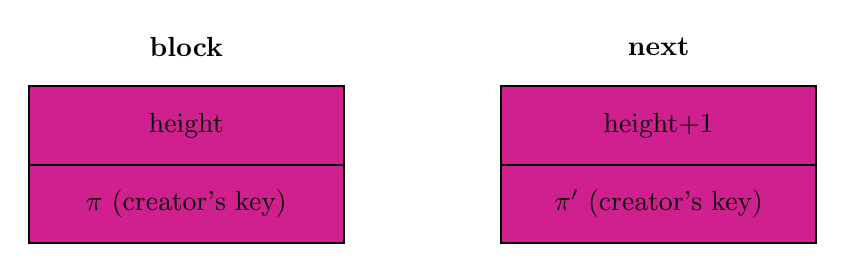
\begin{tikzpicture}
      \draw (2,7) node{\textbf{block}};
      \draw [fill=VioletRed, thick] (0,5.5) rectangle (4,6.5);
      \draw (2,6) node{height};
      \draw [fill=VioletRed, thick] (0,4.5) rectangle (4,5.5);
      \draw (2,5) node{$\pi$ (creator's key)};

      \draw (8,7) node{\textbf{next}};
      \draw [fill=VioletRed, thick] (6,5.5) rectangle (10,6.5);
      \draw (8,6) node{height+1};

      \draw [fill=VioletRed, thick] (6,4.5) rectangle (10,5.5);
      \draw (8,5) node{$\pi'$ (creator's key)};
    \end{tikzpicture}
  \end{center}

  Challenge-grinding attacks are only possible if a miner grinds over many impersonations $\pi'$, but:

  \begin{enumerate}
    \pause
  \item this requires to recompute nonces on-the-fly for each impersonation: very expensive
    \pause
  \item this requires to recollect mining fees from all used impersonations: complicated
    and expensive (transfer fees)
  \end{enumerate}

  \pause
  \begin{center}
    \textbf{Proposition.} Signum is largely protected from challenge-grinding attacks
  \end{center}

\end{frame}

\addtocounter{framenumber}{-1}

\begin{frame}\frametitle{Protection against newborn attacks}

  \begin{redbox}{Problem: the same plot file can be used for mining for many distinct blockchain
      networks using the Signum protocol}
    Who has allocated a big plot file for an established network can use it for free
    for mining \textbf{(concurrently!)} for another, newborn, small network and effectively take its control!
  \end{redbox}

  \medskip

  \begin{center}
    Expensive with PoW: CPU power can only be used for a single network
  \end{center}

  \bigskip

  \visible<2->{
  \begin{greenbox}{Solution}
    Enrich $\pi$ (the block creator's key) with extra information about
    \begin{itemize}
    \item chain name
    \item chain id
    \item genesis time
    \item \ldots
    \end{itemize}
    Add a consensus rule that checks such extra data
  \end{greenbox}
  }

\end{frame}

\addtocounter{framenumber}{-1}

\begin{frame}\frametitle{Protection against censorship attacks}

  \begin{center}
    \begin{tikzpicture}
      \draw [decorate,decoration={brace,amplitude=4pt},thick,xshift=0.3cm,yshift=0pt]
      (6,6.5) -- (6,4.5) node [midway,right,xshift=.2cm] {trunk};
      \draw [fill=VioletRed, thick] (0,4.5) rectangle (6,6.5);
      \draw (3,6) node{height};
      \draw [fill=VioletRed, thick] (0,3.5) rectangle (6,5.5);
      \draw (3,5) node{$\pi$ (creator's key)};
      \draw [fill=Yellow, thick] (0,3.5) rectangle (6,4.5);
      \draw (3,4) node{$\previousblockhash$};
      \draw[->,thick] (0,4) -- (-1,4) node [midway,left,xshift=-.5cm] {$\previous$};

      \draw [fill=Yellow, thick] (0,2.5) rectangle (6,3.5);
      \draw (3,3) node{nonce};
      \draw [fill=Yellow, thick] (0,1.5) rectangle (6,2.5);
      \draw (3,2) node{$\tau$ (creation time)};

      \draw [fill=SpringGreen, thick] (0,0.5) rectangle (6,1.5);
      \only<1,3>{\draw (3,1) node{\textbf{\Large $\Rightarrow$transactions$\Leftarrow$}};}
      \only<2>{\draw (3,1) node{\textbf{\Large $\Rightarrow$censored transactions$\Leftarrow$}};}

      \visible<3>{
      \draw [fill=SkyBlue, thick] (0,-0.5) rectangle (6,0.5);
      \draw (3,0) node{$\pi$'s signature};
      }

    \end{tikzpicture}
  \end{center}

  \begin{center}
    \only<1>{Transactions are not used for mining}
    \only<2>{Transactions can be replaced by any set of censored transactions!}
    \only<3>{Solution: sign with $\pi$'s private key and add a consensus rule to check it}
  \end{center}

\end{frame}

\addtocounter{framenumber}{-1}

\begin{frame}{Optimization: deadlines instead of nonces}

  \begin{center}
    \begin{tikzpicture}
      \draw [decorate,decoration={brace,amplitude=4pt},thick,xshift=0.3cm,yshift=0pt]
      (4,6.5) -- (4,4.5) node [midway,right,xshift=.2cm] {trunk};
      \draw [fill=VioletRed, thick] (0,4.5) rectangle (4,6.5);
      \draw (2,6) node{height};
      \draw [fill=VioletRed, thick] (0,3.5) rectangle (4,5.5);
      \draw (2,5) node{$\pi$ (creator's key)};
      \draw [fill=Yellow, thick] (0,3.5) rectangle (4,4.5);
      \draw (2,4) node{$\previousblockhash$};
      \draw[->,thick] (0,4) -- (-1,4) node [midway,left,xshift=-.5cm] {$\previous$};

      \draw [fill=Yellow, thick] (0,2.5) rectangle (4,3.5);
      \only<1>{\draw (2,3) node{\textbf{\Large $\Rightarrow$nonce$\Leftarrow$}};}
      \only<2>{\draw (2,3) node{\textbf{\Large $\Rightarrow$deadline$\Leftarrow$}};}
      \draw [fill=Yellow, thick] (0,1.5) rectangle (4,2.5);
      \draw (2,2) node{$\tau$ (creation time)};

      \draw [fill=SpringGreen, thick] (0,0.5) rectangle (4,1.5);
      \draw (2,1) node{transactions};
      \draw [fill=SkyBlue, thick] (0,-0.5) rectangle (4,0.5);
      \draw (2,0) node{$\pi$'s signature};
    \end{tikzpicture}
  \end{center}

  \begin{center}
    \only<1>{A nonce is too big for each block ($262$ Kbytes)}
    \only<2>{Replace it with a compact representation called deadline ($200$ bytes)}
  \end{center}

\end{frame}

\end{document}
